\chapter{System Implementation and Application}
\label{chap:ch7}

\section{System Overview}

This chapter describes the design, implementation, and testing of the interactive web application built to demonstrate the 3D fracture assembly models developed in this thesis. The application allows users to select fractured objects, choose between different model variants (baseline, pair attention, double attention), and visualize both the broken fragments and the assembled result in real-time 3D viewers.

The system is structured as a \textbf{two-server architecture}: a Django web application that serves the user interface and manages static assets, and a FastAPI inference server that runs on a GPU-equipped machine and performs model inference. When the GPU server is unavailable, the application falls back to precomputed results, ensuring the demo remains functional without dedicated hardware.

\section{System Architecture}

The application follows a client-server architecture with a clear separation between presentation, orchestration, and computation. Figure~\ref{fig:app_architecture} illustrates the overall system design.

\begin{figure}[H]
    \centering
    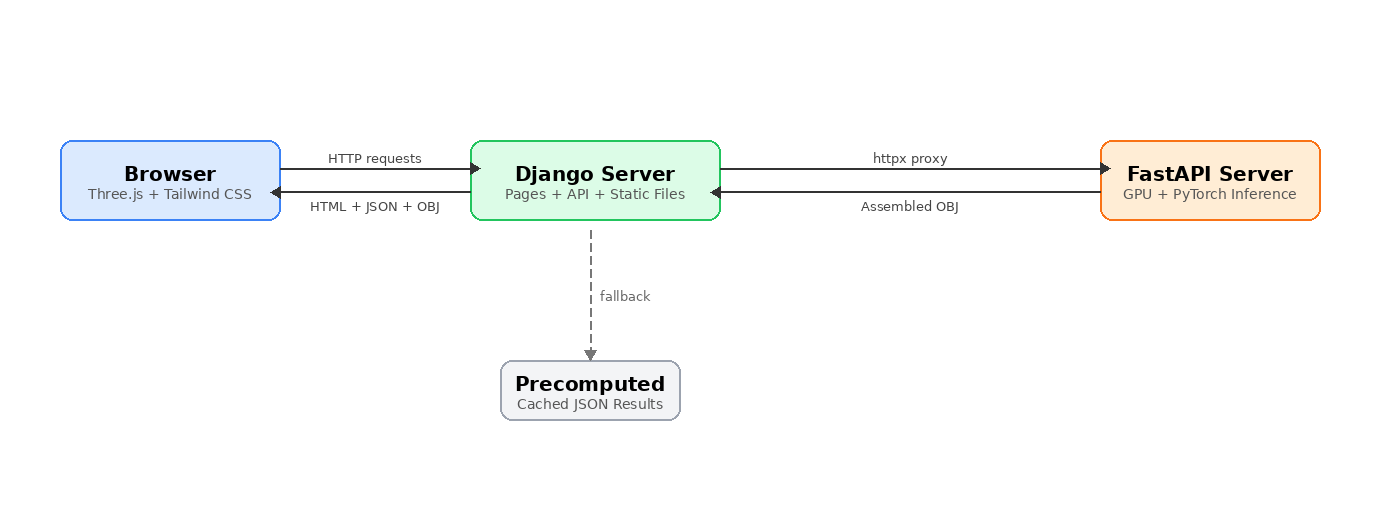
\includegraphics[width=0.9\linewidth]{figures/app_architecture.png}
    \caption{System architecture. The Django server handles user requests and serves static assets. Inference requests are proxied to the FastAPI GPU server when available, with automatic fallback to precomputed results.}
    \label{fig:app_architecture}
\end{figure}


\subsection{Django Web Server}

The Django application (Django 6.0) serves as the main entry point for users. It is responsible for:

\begin{itemize}
    \item \textbf{Page rendering:} Server-side rendering of the main page, including thesis summary slides and the interactive demo panel.
    \item \textbf{Static asset serving:} Hosting the 3D mesh files (Wavefront OBJ format) for all predefined fracture examples, organized by category and piece count.
    \item \textbf{API endpoints:} A REST-style JSON API for fracture metadata retrieval and inference orchestration.
    \item \textbf{Inference proxying:} Forwarding prediction requests to the GPU server via HTTP, with automatic fallback to a precomputed results cache.
\end{itemize}

The Django server exposes three endpoints:

\begin{itemize}
    \item \texttt{GET /} --- Renders the main page with fracture lists injected into the template context.
    \item \texttt{GET /api/fracture/<id>/} --- Returns JSON metadata and static OBJ URLs for a specific fracture.
    \item \texttt{POST /api/predict/} --- Accepts a fracture ID and model variant, proxies to the GPU server or returns cached results.
\end{itemize}

\subsection{FastAPI Inference Server}

The inference server is a separate FastAPI application designed to run on a GPU-equipped machine. It exposes:

\begin{itemize}
    \item \texttt{GET /health} --- Returns server status and CUDA availability.
    \item \texttt{GET /models} --- Lists all six available model variants with descriptions and maximum piece counts.
    \item \texttt{POST /predict} --- Accepts OBJ files as multipart uploads, runs the full Jigsaw inference pipeline (preprocessing, forward pass, global alignment), and returns the assembled meshes as OBJ text.
\end{itemize}

The server validates all inputs: it rejects requests with fewer than 2 pieces, more pieces than the selected model supports (2 for two-piece models, 4 for multi-piece), and files that are not valid UTF-8 text.

\subsection{Fallback Mechanism}

The predict endpoint implements a three-tier fallback strategy:

\begin{enumerate}
    \item \textbf{Live GPU inference:} If the \texttt{GPU\_POD\_URL} environment variable is configured and the server is reachable, the request is proxied using \texttt{httpx} with a 120-second timeout.
    \item \textbf{Precomputed cache:} If the GPU is unreachable, the system looks up the result in a static JSON file (\texttt{precomputed\_results.json}) indexed by fracture ID and model variant.
    \item \textbf{Error response:} If neither source is available, the system returns HTTP 503 with a descriptive error message.
\end{enumerate}

This design ensures the demo functions reliably during presentations and evaluations without requiring a dedicated GPU server.

\section{Technologies}

Table~\ref{tab:technologies} summarizes the technology stack used in the application.

\begin{table}[H]
\centering
\caption{Technology stack.}
\label{tab:technologies}
\begin{tabular}{ll}
\toprule
\textbf{Component} & \textbf{Technology} \\
\midrule
Web framework & Django 6.0 \\
Inference server & FastAPI + Uvicorn \\
Deep learning & PyTorch + PyTorch Lightning \\
3D visualization & Three.js r170 (ES modules) \\
CSS framework & Tailwind CSS (CDN) \\
Point cloud processing & PyTorch Geometric, Open3D, Trimesh \\
Pose optimization & GTSAM (Shonan averaging) \\
HTTP client & httpx (Django $\to$ FastAPI proxy) \\
\bottomrule
\end{tabular}
\end{table}

\section{Data Organization}

Fracture examples are stored as static OBJ files organized in a hierarchical directory structure:

\begin{verbatim}
meshes/
  two_pieces/
    <category>/
      <mesh_hash>/
        fractured_0/
          piece_0.obj
          piece_1.obj
  multi_pieces/
    <category>/
      <mesh_hash>/
        fractured_0/
          piece_0.obj
          piece_1.obj
          piece_2.obj
\end{verbatim}

At startup, the Django application automatically discovers all valid fractures by walking this directory tree. Each fracture is assigned a deterministic 12-character ID derived from its path, ensuring stable URLs across restarts. The discovery logic filters for directories starting with \texttt{fractured\_} and containing at least two \texttt{piece\_*.obj} files.

\section{User Interface}

The application presents a single-page layout consisting of two main regions: a scrollable narrative column on the left and a sticky interactive demo panel on the right.

\subsection{Narrative Slides}

The left column contains five full-viewport-height slides summarizing the thesis:

\begin{enumerate}
    \item \textbf{Problem introduction:} Fracture assembly as a 6-DoF pose estimation problem, applications in archaeology and forensics.
    \item \textbf{Jigsaw pipeline:} Overview of the four-stage architecture (PointNet++, attention, matching, alignment).
    \item \textbf{Proposed improvements:} Pair geometric attention and gated double attention mechanisms.
    \item \textbf{Experimental results:} Key findings on dataset size, architectural modifications, and ICP refinement.
    \item \textbf{Future work:} Scaling to more pieces, loss scheduling, sim-to-real transfer.
\end{enumerate}

Users navigate between slides using arrow buttons or by scrolling.

\subsection{Interactive Demo Panel}

The demo panel remains fixed on the right side of the screen and contains:

\begin{itemize}
    \item \textbf{Model selector:} A dropdown menu listing all six model variants (baseline, pair attention, double attention $\times$ two-piece and multi-piece).
    \item \textbf{Category filter:} Filters the available examples by object category (e.g., BeerBottle, Cup).
    \item \textbf{Example navigator:} Previous/next buttons and a counter to browse through examples within the selected category.
    \item \textbf{Input viewer:} A 3D viewer displaying the broken fragments in a scattered configuration.
    \item \textbf{Fix Object button:} Triggers inference and displays a loading indicator during processing.
    \item \textbf{Output viewer:} A 3D viewer displaying the assembled result after inference completes.
\end{itemize}

An \textbf{Expand Demo} button opens a fullscreen overlay with a larger 3D viewer and two additional tabs: \textbf{Browse Examples} (a grid of all available fractures with thumbnail cards) and \textbf{Compare Performance} (a side-by-side comparison interface).

\subsection{3D Visualization}

The 3D viewers are built with Three.js (version r170) using ES module imports. Each viewer creates a scene with ambient and directional lighting, a perspective camera with automatic field-of-view fitting, and orbit controls for rotation, zoom, and pan. Fragment meshes are parsed from OBJ text using Three.js's \texttt{OBJLoader} and rendered with flat shading. Each piece is assigned a distinct color to visually distinguish fragments, and in the input viewer, pieces are scattered outward from their shared centroid to prevent overlap.

\section{User Manual}

This section describes the step-by-step workflow for using the application.

% TODO: Add screenshots for each step
\subsection{Step 1: Launch and Overview}

Upon opening the application, the user is presented with a hero section introducing the thesis topic. Scrolling down or clicking \textbf{Explore the Demo} reveals the main content area with narrative slides on the left and the interactive demo on the right.

\begin{figure}[H]
    \centering
    \includegraphics[width=0.85\linewidth]{figures/hero_landing_page.png}
    \caption{Landing page with hero section and call-to-action button.}
    \label{fig:app_hero}
\end{figure}


\subsection{Step 2: Select a Model and View Fragments}

The user selects a model variant from the dropdown (e.g., ``Baseline (2 pieces)'' or ``Double attention (2-4 pieces)''). The category filter narrows the list of available examples, and the previous/next buttons or the fullscreen grid allow browsing. After selecting an example, the input viewer loads and displays the fragment meshes in a scattered arrangement with distinct colors, allowing inspection via rotation, zoom, and pan.

\begin{figure}
    \centering
    \includegraphics[width=0.85\linewidth]{figures/app_select.png}
    \caption{Example selection interface with model dropdown, category filter, and broken fragments displayed in the 3D input viewer.}
    \label{fig:app_select}
\end{figure}

\subsection{Step 3: Run Inference}

Clicking the \textbf{Fix Object} button triggers the inference process. The button displays a loading animation while the request is processed. The system either performs live inference on the GPU server or retrieves a cached result. A status message indicates the source of the result (live or cached).

\begin{figure}[H]
    \centering
    \includegraphics[width=0.85\linewidth]{figures/app_result.png}
    \caption{Assembled result displayed in the output viewer after clicking Fix Object. The status bar indicates whether the result was computed live or retrieved from cache.}
    \label{fig:app_result}
\end{figure}

\subsection{Step 4: Inspect and Compare}

The output viewer displays the assembled object. The user can rotate and zoom to inspect alignment quality (Figure~\ref{fig:inspect_result}). Switching to a different model variant and clicking Fix Object again allows comparing reconstruction quality across architectures. The \textbf{Expand Demo} button opens a fullscreen overlay with a larger viewer and a \textbf{Browse Examples} grid for quick selection (Figure~\ref{fig:app_fullscreen}).

\begin{figure}[H]
    \centering
    \begin{subfigure}[t]{0.48\linewidth}
        \centering
        \includegraphics[width=\linewidth]{figures/show_zoom.png}
        \caption{Zoomed view of the assembled object.}
    \end{subfigure}
    \hfill
    \begin{subfigure}[t]{0.48\linewidth}
        \centering
        \includegraphics[width=\linewidth]{figures/show_zoom_rotation.png}
        \caption{Close-up inspection of the fracture pattern.}
    \end{subfigure}
    \caption{Detailed inspection of the reconstruction result from different viewing angles.}
    \label{fig:inspect_result}
\end{figure}

\begin{figure}[H]
    \centering
    \includegraphics[width=0.75\linewidth]{figures/app_fullscreen.png}
    \caption{Fullscreen demo view with the Browse Examples grid for quick selection.}
    \label{fig:app_fullscreen}
\end{figure}

\section{Functional Requirements}

The application satisfies the following functional requirements:

\begin{itemize}
    \item \textbf{F1 -- Fracture visualization:} Display broken 3D fragments in an interactive viewer with rotation, zoom, and pan controls.
    \item \textbf{F2 -- Model selection:} Allow the user to choose between six model variants covering different architectural configurations and piece counts.
    \item \textbf{F3 -- Inference execution:} Perform end-to-end fracture assembly inference (feature extraction, segmentation, matching, and global alignment) given a set of OBJ fragments.
    \item \textbf{F4 -- Result visualization:} Display the assembled object in a separate 3D viewer for inspection.
    \item \textbf{F5 -- Graceful degradation:} Operate without a GPU server by serving precomputed results from a static cache.
    \item \textbf{F6 -- Example browsing:} Provide navigation controls and a fullscreen grid for browsing the complete set of available examples.
\end{itemize}

\section{Non-Functional Requirements}

\begin{itemize}
    \item \textbf{Performance:} Live inference completes within 120 seconds (the proxy timeout). Precomputed fallback responses are served in under 100ms.
    \item \textbf{Portability:} The Django server runs on any Linux environment with Python 3.12+. The inference server requires CUDA-capable hardware with at least 8 GB VRAM.
    \item \textbf{Maintainability:} The codebase is modular: data processing, model components, training infrastructure, web application, and inference server are clearly separated. Configuration is externalized through environment variables and YAML files.
    \item \textbf{Security:} CSRF protection is enabled on all POST endpoints. Session cookies are configured with \texttt{HttpOnly} and \texttt{SameSite=Lax} flags. The inference server restricts CORS origins via environment configuration.
\end{itemize}

\section{Constraints and Assumptions}

The system assumes that all fragments are rigid bodies with no deformation or material loss, and that they belong to a single object forming a complete reconstruction. The dataset consists of synthetically generated fractures with clean geometric surfaces. GPU acceleration is required for live inference, and memory usage scales quadratically with point count due to the attention and matching stages. The application focuses on demonstrating pretrained models rather than exposing training functionality.

\section{Testing}

The application is covered by automated tests at two levels: the Django web layer and the FastAPI inference server. All tests run without GPU access by mocking heavy dependencies (PyTorch, model inference), ensuring they can be executed in any development environment.

Table~\ref{tab:test_summary} summarizes the test coverage across both components. The Django tests use the built-in \texttt{django.test} framework, while the FastAPI tests use \texttt{pytest} with FastAPI's \texttt{TestClient}. All 27 tests pass successfully and run without GPU access by mocking heavy dependencies.

\begin{table}[H]
\centering
\caption{Test suite summary. All tests run without GPU by mocking PyTorch and model inference.}
\label{tab:test_summary}
\begin{tabular}{llr}
\toprule
\textbf{Component} & \textbf{Test Layer} & \textbf{Tests} \\
\midrule
Django & Data model (ID generation, display names, paths) & 5 \\
Django & View layer (page rendering, JSON API, 404 handling) & 5 \\
Django & Integration (GPU proxy, cache fallback, 503 error) & 4 \\
\midrule
FastAPI & Health and model listing & 7 \\
FastAPI & Input validation (piece count, UTF-8, model variant) & 5 \\
FastAPI & End-to-end inference (mocked) & 1 \\
\midrule
& \textbf{Total} & \textbf{27} \\
\bottomrule
\end{tabular}
\end{table}
